\section{Einführung}
\section{Versuch}
Im Folgendem werden die Kennlienen von verschieden Bauteilen mit dem Aufbau \ref{fig:aufbau} bestimmt.
\begin{figure}[H]
	\centering
	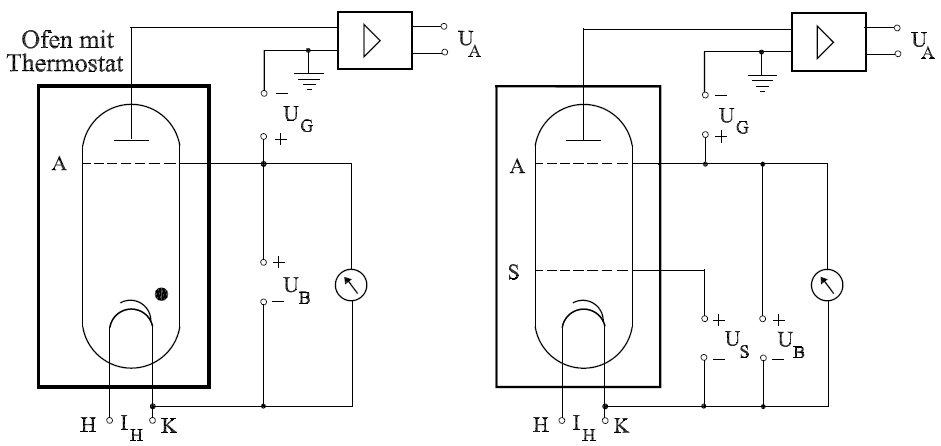
\includegraphics[width=.8\textwidth]{aufbau.png}
	\caption{Messaufbau für unterschiedliche Leiter}
	\label{fig:aufbau}
\end{figure}
\subsection{Diode in Durchlassrichtung}
Wie in Abbildung \ref{fig:aufbau} a) gezeigt wird der Strom für unterschiedliche Spannung gemessen, um daraus eine U-I-Kennlinie zu ermitteln.

\begin{figure}[H]
\centering
% GNUPLOT: LaTeX picture
\setlength{\unitlength}{0.240900pt}
\ifx\plotpoint\undefined\newsavebox{\plotpoint}\fi
\begin{picture}(1500,900)(0,0)
\sbox{\plotpoint}{\rule[-0.200pt]{0.400pt}{0.400pt}}%
\put(151.0,131.0){\rule[-0.200pt]{4.818pt}{0.400pt}}
\put(131,131){\makebox(0,0)[r]{ 0}}
\put(1419.0,131.0){\rule[-0.200pt]{4.818pt}{0.400pt}}
\put(151.0,252.0){\rule[-0.200pt]{4.818pt}{0.400pt}}
\put(131,252){\makebox(0,0)[r]{ 10}}
\put(1419.0,252.0){\rule[-0.200pt]{4.818pt}{0.400pt}}
\put(151.0,374.0){\rule[-0.200pt]{4.818pt}{0.400pt}}
\put(131,374){\makebox(0,0)[r]{ 20}}
\put(1419.0,374.0){\rule[-0.200pt]{4.818pt}{0.400pt}}
\put(151.0,495.0){\rule[-0.200pt]{4.818pt}{0.400pt}}
\put(131,495){\makebox(0,0)[r]{ 30}}
\put(1419.0,495.0){\rule[-0.200pt]{4.818pt}{0.400pt}}
\put(151.0,616.0){\rule[-0.200pt]{4.818pt}{0.400pt}}
\put(131,616){\makebox(0,0)[r]{ 40}}
\put(1419.0,616.0){\rule[-0.200pt]{4.818pt}{0.400pt}}
\put(151.0,738.0){\rule[-0.200pt]{4.818pt}{0.400pt}}
\put(131,738){\makebox(0,0)[r]{ 50}}
\put(1419.0,738.0){\rule[-0.200pt]{4.818pt}{0.400pt}}
\put(151.0,859.0){\rule[-0.200pt]{4.818pt}{0.400pt}}
\put(131,859){\makebox(0,0)[r]{ 60}}
\put(1419.0,859.0){\rule[-0.200pt]{4.818pt}{0.400pt}}
\put(151.0,131.0){\rule[-0.200pt]{0.400pt}{4.818pt}}
\put(151,90){\makebox(0,0){ 0}}
\put(151.0,839.0){\rule[-0.200pt]{0.400pt}{4.818pt}}
\put(312.0,131.0){\rule[-0.200pt]{0.400pt}{4.818pt}}
\put(312,90){\makebox(0,0){ 0.1}}
\put(312.0,839.0){\rule[-0.200pt]{0.400pt}{4.818pt}}
\put(473.0,131.0){\rule[-0.200pt]{0.400pt}{4.818pt}}
\put(473,90){\makebox(0,0){ 0.2}}
\put(473.0,839.0){\rule[-0.200pt]{0.400pt}{4.818pt}}
\put(634.0,131.0){\rule[-0.200pt]{0.400pt}{4.818pt}}
\put(634,90){\makebox(0,0){ 0.3}}
\put(634.0,839.0){\rule[-0.200pt]{0.400pt}{4.818pt}}
\put(795.0,131.0){\rule[-0.200pt]{0.400pt}{4.818pt}}
\put(795,90){\makebox(0,0){ 0.4}}
\put(795.0,839.0){\rule[-0.200pt]{0.400pt}{4.818pt}}
\put(956.0,131.0){\rule[-0.200pt]{0.400pt}{4.818pt}}
\put(956,90){\makebox(0,0){ 0.5}}
\put(956.0,839.0){\rule[-0.200pt]{0.400pt}{4.818pt}}
\put(1117.0,131.0){\rule[-0.200pt]{0.400pt}{4.818pt}}
\put(1117,90){\makebox(0,0){ 0.6}}
\put(1117.0,839.0){\rule[-0.200pt]{0.400pt}{4.818pt}}
\put(1278.0,131.0){\rule[-0.200pt]{0.400pt}{4.818pt}}
\put(1278,90){\makebox(0,0){ 0.7}}
\put(1278.0,839.0){\rule[-0.200pt]{0.400pt}{4.818pt}}
\put(1439.0,131.0){\rule[-0.200pt]{0.400pt}{4.818pt}}
\put(1439,90){\makebox(0,0){ 0.8}}
\put(1439.0,839.0){\rule[-0.200pt]{0.400pt}{4.818pt}}
\put(151.0,131.0){\rule[-0.200pt]{0.400pt}{175.375pt}}
\put(151.0,131.0){\rule[-0.200pt]{310.279pt}{0.400pt}}
\put(1439.0,131.0){\rule[-0.200pt]{0.400pt}{175.375pt}}
\put(151.0,859.0){\rule[-0.200pt]{310.279pt}{0.400pt}}
\put(30,495){\makebox(0,0){I [mA]}}
\put(795,29){\makebox(0,0){U [mV]}}
\put(156,131){\makebox(0,0){$+$}}
\put(190,131){\makebox(0,0){$+$}}
\put(431,131){\makebox(0,0){$+$}}
\put(550,131){\makebox(0,0){$+$}}
\put(592,131){\makebox(0,0){$+$}}
\put(658,131){\makebox(0,0){$+$}}
\put(710,131){\makebox(0,0){$+$}}
\put(776,131){\makebox(0,0){$+$}}
\put(826,131){\makebox(0,0){$+$}}
\put(888,132){\makebox(0,0){$+$}}
\put(938,133){\makebox(0,0){$+$}}
\put(987,135){\makebox(0,0){$+$}}
\put(1074,149){\makebox(0,0){$+$}}
\put(1115,167){\makebox(0,0){$+$}}
\put(1162,208){\makebox(0,0){$+$}}
\put(1214,305){\makebox(0,0){$+$}}
\put(1278,628){\makebox(0,0){$+$}}
\put(1299,821){\makebox(0,0){$+$}}
\put(156,131){\usebox{\plotpoint}}
\put(156.00,131.00){\usebox{\plotpoint}}
\put(176.76,131.00){\usebox{\plotpoint}}
\put(197.51,131.00){\usebox{\plotpoint}}
\put(218.27,131.00){\usebox{\plotpoint}}
\put(239.02,131.00){\usebox{\plotpoint}}
\put(259.78,131.00){\usebox{\plotpoint}}
\put(280.53,131.00){\usebox{\plotpoint}}
\put(301.29,131.00){\usebox{\plotpoint}}
\put(322.04,131.00){\usebox{\plotpoint}}
\put(342.80,131.00){\usebox{\plotpoint}}
\put(363.55,131.00){\usebox{\plotpoint}}
\put(384.31,131.00){\usebox{\plotpoint}}
\put(405.07,131.00){\usebox{\plotpoint}}
\put(425.82,131.00){\usebox{\plotpoint}}
\put(446.58,131.00){\usebox{\plotpoint}}
\put(467.33,131.00){\usebox{\plotpoint}}
\put(488.09,131.00){\usebox{\plotpoint}}
\put(508.84,131.00){\usebox{\plotpoint}}
\put(529.60,131.00){\usebox{\plotpoint}}
\put(550.35,131.00){\usebox{\plotpoint}}
\put(571.11,131.00){\usebox{\plotpoint}}
\put(591.87,131.00){\usebox{\plotpoint}}
\put(612.62,131.00){\usebox{\plotpoint}}
\put(633.38,131.00){\usebox{\plotpoint}}
\put(654.13,131.00){\usebox{\plotpoint}}
\put(674.89,131.00){\usebox{\plotpoint}}
\put(695.64,131.00){\usebox{\plotpoint}}
\put(716.40,131.00){\usebox{\plotpoint}}
\put(737.15,131.00){\usebox{\plotpoint}}
\put(757.91,131.00){\usebox{\plotpoint}}
\put(778.66,131.00){\usebox{\plotpoint}}
\put(799.42,131.00){\usebox{\plotpoint}}
\put(820.18,131.00){\usebox{\plotpoint}}
\put(840.92,131.33){\usebox{\plotpoint}}
\put(861.65,132.00){\usebox{\plotpoint}}
\put(882.40,132.00){\usebox{\plotpoint}}
\put(903.16,132.00){\usebox{\plotpoint}}
\put(923.87,133.00){\usebox{\plotpoint}}
\put(944.61,133.30){\usebox{\plotpoint}}
\put(965.33,134.11){\usebox{\plotpoint}}
\put(986.01,135.91){\usebox{\plotpoint}}
\put(1006.69,137.70){\usebox{\plotpoint}}
\put(1027.30,139.96){\usebox{\plotpoint}}
\put(1047.76,143.50){\usebox{\plotpoint}}
\put(1068.01,148.00){\usebox{\plotpoint}}
\put(1087.64,154.47){\usebox{\plotpoint}}
\put(1106.57,162.95){\usebox{\plotpoint}}
\put(1124.62,173.19){\usebox{\plotpoint}}
\put(1140.80,186.16){\usebox{\plotpoint}}
\put(1155.51,200.69){\usebox{\plotpoint}}
\put(1168.62,216.78){\usebox{\plotpoint}}
\put(1180.00,234.10){\usebox{\plotpoint}}
\put(1190.19,252.18){\usebox{\plotpoint}}
\put(1199.35,270.78){\usebox{\plotpoint}}
\multiput(1207,288)(6.747,19.628){2}{\usebox{\plotpoint}}
\multiput(1218,320)(6.250,19.792){2}{\usebox{\plotpoint}}
\multiput(1230,358)(4.730,20.209){2}{\usebox{\plotpoint}}
\multiput(1241,405)(4.349,20.295){3}{\usebox{\plotpoint}}
\multiput(1253,461)(3.363,20.481){3}{\usebox{\plotpoint}}
\multiput(1264,528)(3.042,20.531){4}{\usebox{\plotpoint}}
\multiput(1276,609)(2.339,20.623){5}{\usebox{\plotpoint}}
\multiput(1287,706)(2.118,20.647){6}{\usebox{\plotpoint}}
\put(1299,823){\usebox{\plotpoint}}
\put(151.0,131.0){\rule[-0.200pt]{0.400pt}{175.375pt}}
\put(151.0,131.0){\rule[-0.200pt]{310.279pt}{0.400pt}}
\put(1439.0,131.0){\rule[-0.200pt]{0.400pt}{175.375pt}}
\put(151.0,859.0){\rule[-0.200pt]{310.279pt}{0.400pt}}
\end{picture}

\caption{Messwerte und Fit für eine Diode in Durchlassrichtung}
\label{fig:diode}
\end{figure}
Aufgrund des anscheinend exponentiellen Verlaufs der Messwerte wurde mit \emph{gnuplot} nach dem \emph{least-squares}-Verfahren die Werte gegen die Funktion $f(x)=a\cdot b^x$ gefittet. Ausgabe:
\begin{table}[H]
  \centering
  \begin{tabular}{c | c | c }
    Variabel   & Wert & Unsicherheit\\ \hline
    a & $\num{5.61784d-7}$ & $\pm\num{3.084d-8}$ \\
    b & $\num{1.69598d+11}$ & $\pm\num{1.319d+10}$
  \end{tabular}
  \caption{Linearer Fit zu Abbildung \ref{fig:diode}}
  \label{tab:fitdiode}
\end{table}
\subsection{Zenerdiode}
Wie in Abbildung \ref{fig:aufbau} b) gezeigt wird der Strom für unterschiedliche Spannung gemessen, um daraus eine U-I-Kennlinie zu ermitteln. Dies wird jedoch einmal mit einer Polung in Durchlassrichtung und einmal in Sperrrichtung getan.
\begin{figure}[H]
\centering
\input{Diodesperr.tex}
\caption{Messwerte und Fit für eine Zenerdiode in Sperrrichtung}
\label{fig:diodesperr}
\end{figure}
Aufgrund des anscheinend exponentiellen Verlaufs der Messwerte wurde mit \emph{gnuplot} nach dem \emph{least-squares}-Verfahren die Werte gegen die Funktion $f(x)=a\cdot b^x$ gefittet. Ausgabe:
\begin{table}[H]
  \centering
  \begin{tabular}{c | c | c }
    Variabel   & Wert & Unsicherheit\\ \hline
    a & $\num{1.50271d-7}$ & $\pm\num{5.433d-8}$ \\
    b & $\num{42.7533}$ & $\pm\num{3.073}$
  \end{tabular}
  \caption{Linearer Fit zu Abbildung \ref{fig:diodesperr}}
  \label{tab:fitdiodesperr}
\end{table}
\begin{figure}[H]
\centering
% GNUPLOT: LaTeX picture
\setlength{\unitlength}{0.240900pt}
\ifx\plotpoint\undefined\newsavebox{\plotpoint}\fi
\begin{picture}(1500,900)(0,0)
\sbox{\plotpoint}{\rule[-0.200pt]{0.400pt}{0.400pt}}%
\put(151.0,131.0){\rule[-0.200pt]{4.818pt}{0.400pt}}
\put(131,131){\makebox(0,0)[r]{ 0}}
\put(1419.0,131.0){\rule[-0.200pt]{4.818pt}{0.400pt}}
\put(151.0,222.0){\rule[-0.200pt]{4.818pt}{0.400pt}}
\put(131,222){\makebox(0,0)[r]{ 5}}
\put(1419.0,222.0){\rule[-0.200pt]{4.818pt}{0.400pt}}
\put(151.0,313.0){\rule[-0.200pt]{4.818pt}{0.400pt}}
\put(131,313){\makebox(0,0)[r]{ 10}}
\put(1419.0,313.0){\rule[-0.200pt]{4.818pt}{0.400pt}}
\put(151.0,404.0){\rule[-0.200pt]{4.818pt}{0.400pt}}
\put(131,404){\makebox(0,0)[r]{ 15}}
\put(1419.0,404.0){\rule[-0.200pt]{4.818pt}{0.400pt}}
\put(151.0,495.0){\rule[-0.200pt]{4.818pt}{0.400pt}}
\put(131,495){\makebox(0,0)[r]{ 20}}
\put(1419.0,495.0){\rule[-0.200pt]{4.818pt}{0.400pt}}
\put(151.0,586.0){\rule[-0.200pt]{4.818pt}{0.400pt}}
\put(131,586){\makebox(0,0)[r]{ 25}}
\put(1419.0,586.0){\rule[-0.200pt]{4.818pt}{0.400pt}}
\put(151.0,677.0){\rule[-0.200pt]{4.818pt}{0.400pt}}
\put(131,677){\makebox(0,0)[r]{ 30}}
\put(1419.0,677.0){\rule[-0.200pt]{4.818pt}{0.400pt}}
\put(151.0,768.0){\rule[-0.200pt]{4.818pt}{0.400pt}}
\put(131,768){\makebox(0,0)[r]{ 35}}
\put(1419.0,768.0){\rule[-0.200pt]{4.818pt}{0.400pt}}
\put(151.0,859.0){\rule[-0.200pt]{4.818pt}{0.400pt}}
\put(131,859){\makebox(0,0)[r]{ 40}}
\put(1419.0,859.0){\rule[-0.200pt]{4.818pt}{0.400pt}}
\put(151.0,131.0){\rule[-0.200pt]{0.400pt}{4.818pt}}
\put(151,90){\makebox(0,0){ 0}}
\put(151.0,839.0){\rule[-0.200pt]{0.400pt}{4.818pt}}
\put(312.0,131.0){\rule[-0.200pt]{0.400pt}{4.818pt}}
\put(312,90){\makebox(0,0){ 0.1}}
\put(312.0,839.0){\rule[-0.200pt]{0.400pt}{4.818pt}}
\put(473.0,131.0){\rule[-0.200pt]{0.400pt}{4.818pt}}
\put(473,90){\makebox(0,0){ 0.2}}
\put(473.0,839.0){\rule[-0.200pt]{0.400pt}{4.818pt}}
\put(634.0,131.0){\rule[-0.200pt]{0.400pt}{4.818pt}}
\put(634,90){\makebox(0,0){ 0.3}}
\put(634.0,839.0){\rule[-0.200pt]{0.400pt}{4.818pt}}
\put(795.0,131.0){\rule[-0.200pt]{0.400pt}{4.818pt}}
\put(795,90){\makebox(0,0){ 0.4}}
\put(795.0,839.0){\rule[-0.200pt]{0.400pt}{4.818pt}}
\put(956.0,131.0){\rule[-0.200pt]{0.400pt}{4.818pt}}
\put(956,90){\makebox(0,0){ 0.5}}
\put(956.0,839.0){\rule[-0.200pt]{0.400pt}{4.818pt}}
\put(1117.0,131.0){\rule[-0.200pt]{0.400pt}{4.818pt}}
\put(1117,90){\makebox(0,0){ 0.6}}
\put(1117.0,839.0){\rule[-0.200pt]{0.400pt}{4.818pt}}
\put(1278.0,131.0){\rule[-0.200pt]{0.400pt}{4.818pt}}
\put(1278,90){\makebox(0,0){ 0.7}}
\put(1278.0,839.0){\rule[-0.200pt]{0.400pt}{4.818pt}}
\put(1439.0,131.0){\rule[-0.200pt]{0.400pt}{4.818pt}}
\put(1439,90){\makebox(0,0){ 0.8}}
\put(1439.0,839.0){\rule[-0.200pt]{0.400pt}{4.818pt}}
\put(151.0,131.0){\rule[-0.200pt]{0.400pt}{175.375pt}}
\put(151.0,131.0){\rule[-0.200pt]{310.279pt}{0.400pt}}
\put(1439.0,131.0){\rule[-0.200pt]{0.400pt}{175.375pt}}
\put(151.0,859.0){\rule[-0.200pt]{310.279pt}{0.400pt}}
\put(30,495){\makebox(0,0){I [mA]}}
\put(795,29){\makebox(0,0){U [V]}}
\put(151,131){\makebox(0,0){$+$}}
\put(557,131){\makebox(0,0){$+$}}
\put(954,131){\makebox(0,0){$+$}}
\put(993,132){\makebox(0,0){$+$}}
\put(1038,133){\makebox(0,0){$+$}}
\put(1075,135){\makebox(0,0){$+$}}
\put(1104,139){\makebox(0,0){$+$}}
\put(1136,147){\makebox(0,0){$+$}}
\put(1165,161){\makebox(0,0){$+$}}
\put(1193,188){\makebox(0,0){$+$}}
\put(1214,222){\makebox(0,0){$+$}}
\put(1243,314){\makebox(0,0){$+$}}
\put(1296,804){\makebox(0,0){$+$}}
\put(151,131){\usebox{\plotpoint}}
\put(151.00,131.00){\usebox{\plotpoint}}
\put(171.76,131.00){\usebox{\plotpoint}}
\put(192.51,131.00){\usebox{\plotpoint}}
\put(213.27,131.00){\usebox{\plotpoint}}
\put(234.02,131.00){\usebox{\plotpoint}}
\put(254.78,131.00){\usebox{\plotpoint}}
\put(275.53,131.00){\usebox{\plotpoint}}
\put(296.29,131.00){\usebox{\plotpoint}}
\put(317.04,131.00){\usebox{\plotpoint}}
\put(337.80,131.00){\usebox{\plotpoint}}
\put(358.55,131.00){\usebox{\plotpoint}}
\put(379.31,131.00){\usebox{\plotpoint}}
\put(400.07,131.00){\usebox{\plotpoint}}
\put(420.82,131.00){\usebox{\plotpoint}}
\put(441.58,131.00){\usebox{\plotpoint}}
\put(462.33,131.00){\usebox{\plotpoint}}
\put(483.09,131.00){\usebox{\plotpoint}}
\put(503.84,131.00){\usebox{\plotpoint}}
\put(524.60,131.00){\usebox{\plotpoint}}
\put(545.35,131.00){\usebox{\plotpoint}}
\put(566.11,131.00){\usebox{\plotpoint}}
\put(586.87,131.00){\usebox{\plotpoint}}
\put(607.62,131.00){\usebox{\plotpoint}}
\put(628.38,131.00){\usebox{\plotpoint}}
\put(649.13,131.00){\usebox{\plotpoint}}
\put(669.89,131.00){\usebox{\plotpoint}}
\put(690.64,131.00){\usebox{\plotpoint}}
\put(711.40,131.00){\usebox{\plotpoint}}
\put(732.15,131.00){\usebox{\plotpoint}}
\put(752.91,131.00){\usebox{\plotpoint}}
\put(773.66,131.00){\usebox{\plotpoint}}
\put(794.42,131.00){\usebox{\plotpoint}}
\put(815.18,131.00){\usebox{\plotpoint}}
\put(835.93,131.00){\usebox{\plotpoint}}
\put(856.69,131.00){\usebox{\plotpoint}}
\put(877.44,131.00){\usebox{\plotpoint}}
\put(898.20,131.00){\usebox{\plotpoint}}
\put(918.95,131.00){\usebox{\plotpoint}}
\put(939.71,131.00){\usebox{\plotpoint}}
\put(960.46,131.00){\usebox{\plotpoint}}
\put(981.22,131.00){\usebox{\plotpoint}}
\put(1001.95,131.58){\usebox{\plotpoint}}
\put(1022.69,132.00){\usebox{\plotpoint}}
\put(1043.44,132.20){\usebox{\plotpoint}}
\put(1064.16,133.01){\usebox{\plotpoint}}
\put(1084.84,134.74){\usebox{\plotpoint}}
\put(1105.32,138.05){\usebox{\plotpoint}}
\put(1125.70,141.93){\usebox{\plotpoint}}
\put(1145.44,148.22){\usebox{\plotpoint}}
\put(1163.52,158.35){\usebox{\plotpoint}}
\put(1179.48,171.53){\usebox{\plotpoint}}
\put(1193.29,186.99){\usebox{\plotpoint}}
\multiput(1203,202)(9.601,18.402){2}{\usebox{\plotpoint}}
\put(1221.17,242.38){\usebox{\plotpoint}}
\multiput(1226,256)(5.964,19.880){2}{\usebox{\plotpoint}}
\multiput(1238,296)(4.143,20.338){3}{\usebox{\plotpoint}}
\multiput(1249,350)(3.459,20.465){3}{\usebox{\plotpoint}}
\multiput(1261,421)(2.628,20.588){5}{\usebox{\plotpoint}}
\multiput(1273,515)(1.834,20.674){6}{\usebox{\plotpoint}}
\multiput(1284,639)(1.506,20.701){8}{\usebox{\plotpoint}}
\put(1296,804){\usebox{\plotpoint}}
\put(151.0,131.0){\rule[-0.200pt]{0.400pt}{175.375pt}}
\put(151.0,131.0){\rule[-0.200pt]{310.279pt}{0.400pt}}
\put(1439.0,131.0){\rule[-0.200pt]{0.400pt}{175.375pt}}
\put(151.0,859.0){\rule[-0.200pt]{310.279pt}{0.400pt}}
\end{picture}

\caption{Messwerte und Fit für eine Zenerdiode in Durchlassrichtung}
\label{fig:diodedurch}
\end{figure}
Aufgrund des anscheinend exponentiellen Verlaufs der Messwerte wurde mit \emph{gnuplot} nach dem \emph{least-squares}-Verfahren die Werte gegen die Funktion $f(x)=a\cdot b^x$ gefittet. Ausgabe:
\begin{table}[H]
  \centering
  \begin{tabular}{c | c | c }
    Variabel   & Wert & Unsicherheit\\ \hline
    a & $\num{3.08803d-11}$ & $\pm\num{3.759d-12}$ \\
    b & $\num{9,72068d16}$ & $\pm\num{1.673d16}$
  \end{tabular}
  \caption{Linearer Fit zu Abbildung \ref{fig:diodedurch}}
  \label{tab:fitdiodedurch}
\end{table}
\subsection{Glühlampe}
Wie in Abbildung \ref{fig:aufbau} c) gezeigt wird der Strom für unterschiedliche Spannung gemessen, um daraus eine U-I-Kennlinie zu ermitteln.

\begin{figure}[H]
\centering
% GNUPLOT: LaTeX picture
\setlength{\unitlength}{0.240900pt}
\ifx\plotpoint\undefined\newsavebox{\plotpoint}\fi
\begin{picture}(1500,900)(0,0)
\sbox{\plotpoint}{\rule[-0.200pt]{0.400pt}{0.400pt}}%
\put(151.0,131.0){\rule[-0.200pt]{4.818pt}{0.400pt}}
\put(131,131){\makebox(0,0)[r]{ 0}}
\put(1419.0,131.0){\rule[-0.200pt]{4.818pt}{0.400pt}}
\put(151.0,252.0){\rule[-0.200pt]{4.818pt}{0.400pt}}
\put(131,252){\makebox(0,0)[r]{ 10}}
\put(1419.0,252.0){\rule[-0.200pt]{4.818pt}{0.400pt}}
\put(151.0,374.0){\rule[-0.200pt]{4.818pt}{0.400pt}}
\put(131,374){\makebox(0,0)[r]{ 20}}
\put(1419.0,374.0){\rule[-0.200pt]{4.818pt}{0.400pt}}
\put(151.0,495.0){\rule[-0.200pt]{4.818pt}{0.400pt}}
\put(131,495){\makebox(0,0)[r]{ 30}}
\put(1419.0,495.0){\rule[-0.200pt]{4.818pt}{0.400pt}}
\put(151.0,616.0){\rule[-0.200pt]{4.818pt}{0.400pt}}
\put(131,616){\makebox(0,0)[r]{ 40}}
\put(1419.0,616.0){\rule[-0.200pt]{4.818pt}{0.400pt}}
\put(151.0,738.0){\rule[-0.200pt]{4.818pt}{0.400pt}}
\put(131,738){\makebox(0,0)[r]{ 50}}
\put(1419.0,738.0){\rule[-0.200pt]{4.818pt}{0.400pt}}
\put(151.0,859.0){\rule[-0.200pt]{4.818pt}{0.400pt}}
\put(131,859){\makebox(0,0)[r]{ 60}}
\put(1419.0,859.0){\rule[-0.200pt]{4.818pt}{0.400pt}}
\put(151.0,131.0){\rule[-0.200pt]{0.400pt}{4.818pt}}
\put(151,90){\makebox(0,0){ 0}}
\put(151.0,839.0){\rule[-0.200pt]{0.400pt}{4.818pt}}
\put(335.0,131.0){\rule[-0.200pt]{0.400pt}{4.818pt}}
\put(335,90){\makebox(0,0){ 2}}
\put(335.0,839.0){\rule[-0.200pt]{0.400pt}{4.818pt}}
\put(519.0,131.0){\rule[-0.200pt]{0.400pt}{4.818pt}}
\put(519,90){\makebox(0,0){ 4}}
\put(519.0,839.0){\rule[-0.200pt]{0.400pt}{4.818pt}}
\put(703.0,131.0){\rule[-0.200pt]{0.400pt}{4.818pt}}
\put(703,90){\makebox(0,0){ 6}}
\put(703.0,839.0){\rule[-0.200pt]{0.400pt}{4.818pt}}
\put(887.0,131.0){\rule[-0.200pt]{0.400pt}{4.818pt}}
\put(887,90){\makebox(0,0){ 8}}
\put(887.0,839.0){\rule[-0.200pt]{0.400pt}{4.818pt}}
\put(1071.0,131.0){\rule[-0.200pt]{0.400pt}{4.818pt}}
\put(1071,90){\makebox(0,0){ 10}}
\put(1071.0,839.0){\rule[-0.200pt]{0.400pt}{4.818pt}}
\put(1255.0,131.0){\rule[-0.200pt]{0.400pt}{4.818pt}}
\put(1255,90){\makebox(0,0){ 12}}
\put(1255.0,839.0){\rule[-0.200pt]{0.400pt}{4.818pt}}
\put(1439.0,131.0){\rule[-0.200pt]{0.400pt}{4.818pt}}
\put(1439,90){\makebox(0,0){ 14}}
\put(1439.0,839.0){\rule[-0.200pt]{0.400pt}{4.818pt}}
\put(151.0,131.0){\rule[-0.200pt]{0.400pt}{175.375pt}}
\put(151.0,131.0){\rule[-0.200pt]{310.279pt}{0.400pt}}
\put(1439.0,131.0){\rule[-0.200pt]{0.400pt}{175.375pt}}
\put(151.0,859.0){\rule[-0.200pt]{310.279pt}{0.400pt}}
\put(30,495){\makebox(0,0){I [mA]}}
\put(795,29){\makebox(0,0){U [V]}}
\put(151,131){\makebox(0,0){$+$}}
\put(178,219){\makebox(0,0){$+$}}
\put(207,257){\makebox(0,0){$+$}}
\put(261,310){\makebox(0,0){$+$}}
\put(234,285){\makebox(0,0){$+$}}
\put(288,331){\makebox(0,0){$+$}}
\put(317,353){\makebox(0,0){$+$}}
\put(342,371){\makebox(0,0){$+$}}
\put(372,392){\makebox(0,0){$+$}}
\put(400,410){\makebox(0,0){$+$}}
\put(427,427){\makebox(0,0){$+$}}
\put(527,485){\makebox(0,0){$+$}}
\put(615,531){\makebox(0,0){$+$}}
\put(706,575){\makebox(0,0){$+$}}
\put(886,655){\makebox(0,0){$+$}}
\put(1071,730){\makebox(0,0){$+$}}
\put(1305,817){\makebox(0,0){$+$}}
\put(151,137){\usebox{\plotpoint}}
\multiput(151,137)(4.137,20.339){3}{\usebox{\plotpoint}}
\multiput(163,196)(8.087,19.115){2}{\usebox{\plotpoint}}
\put(181.61,235.32){\usebox{\plotpoint}}
\put(192.87,252.73){\usebox{\plotpoint}}
\put(205.01,269.56){\usebox{\plotpoint}}
\put(218.12,285.64){\usebox{\plotpoint}}
\put(232.07,301.00){\usebox{\plotpoint}}
\put(246.71,315.71){\usebox{\plotpoint}}
\put(261.85,329.88){\usebox{\plotpoint}}
\put(277.44,343.58){\usebox{\plotpoint}}
\put(293.80,356.33){\usebox{\plotpoint}}
\put(310.10,369.16){\usebox{\plotpoint}}
\put(326.77,381.52){\usebox{\plotpoint}}
\put(343.87,393.27){\usebox{\plotpoint}}
\put(361.00,405.00){\usebox{\plotpoint}}
\put(378.66,415.89){\usebox{\plotpoint}}
\put(396.13,427.07){\usebox{\plotpoint}}
\put(414.24,437.22){\usebox{\plotpoint}}
\put(432.18,447.65){\usebox{\plotpoint}}
\put(450.27,457.82){\usebox{\plotpoint}}
\put(468.65,467.45){\usebox{\plotpoint}}
\put(487.06,477.03){\usebox{\plotpoint}}
\put(505.54,486.48){\usebox{\plotpoint}}
\put(523.98,495.99){\usebox{\plotpoint}}
\put(542.79,504.70){\usebox{\plotpoint}}
\put(561.65,513.32){\usebox{\plotpoint}}
\put(580.38,522.26){\usebox{\plotpoint}}
\put(599.34,530.67){\usebox{\plotpoint}}
\put(618.13,539.47){\usebox{\plotpoint}}
\put(637.18,547.72){\usebox{\plotpoint}}
\put(656.30,555.79){\usebox{\plotpoint}}
\put(675.31,564.10){\usebox{\plotpoint}}
\put(694.79,571.24){\usebox{\plotpoint}}
\put(713.90,579.30){\usebox{\plotpoint}}
\put(733.27,586.70){\usebox{\plotpoint}}
\put(752.63,594.18){\usebox{\plotpoint}}
\put(772.07,601.39){\usebox{\plotpoint}}
\put(791.43,608.81){\usebox{\plotpoint}}
\put(810.72,616.44){\usebox{\plotpoint}}
\put(830.37,623.12){\usebox{\plotpoint}}
\put(849.96,629.98){\usebox{\plotpoint}}
\put(869.31,637.44){\usebox{\plotpoint}}
\put(888.90,644.30){\usebox{\plotpoint}}
\put(908.49,651.16){\usebox{\plotpoint}}
\put(928.18,657.73){\usebox{\plotpoint}}
\put(947.76,664.59){\usebox{\plotpoint}}
\put(967.71,670.26){\usebox{\plotpoint}}
\put(987.30,677.10){\usebox{\plotpoint}}
\put(1006.95,683.80){\usebox{\plotpoint}}
\put(1026.85,689.62){\usebox{\plotpoint}}
\put(1046.45,696.44){\usebox{\plotpoint}}
\put(1066.39,702.13){\usebox{\plotpoint}}
\put(1086.04,708.76){\usebox{\plotpoint}}
\put(1105.93,714.64){\usebox{\plotpoint}}
\put(1125.81,720.60){\usebox{\plotpoint}}
\put(1145.73,726.35){\usebox{\plotpoint}}
\put(1165.61,732.20){\usebox{\plotpoint}}
\put(1185.44,738.30){\usebox{\plotpoint}}
\put(1205.26,744.44){\usebox{\plotpoint}}
\put(1225.32,749.77){\usebox{\plotpoint}}
\put(1245.18,755.78){\usebox{\plotpoint}}
\put(1265.15,761.38){\usebox{\plotpoint}}
\put(1285.11,767.03){\usebox{\plotpoint}}
\put(1304.97,772.99){\usebox{\plotpoint}}
\put(1305,773){\usebox{\plotpoint}}
\put(151.0,131.0){\rule[-0.200pt]{0.400pt}{175.375pt}}
\put(151.0,131.0){\rule[-0.200pt]{310.279pt}{0.400pt}}
\put(1439.0,131.0){\rule[-0.200pt]{0.400pt}{175.375pt}}
\put(151.0,859.0){\rule[-0.200pt]{310.279pt}{0.400pt}}
\end{picture}

\caption{Messwerte und Fit für eine Lampe}
\label{fig:Lampe}
\end{figure}
Aufgrund des anscheinend Wurzel artigem Verlaufs der Messwerte, besonders im Bereich bis $3V$, wurde mit \emph{gnuplot} nach dem \emph{least-squares}-Verfahren die Werte gegen die Funktion $f(x)=a\cdot\sqrt{x}$ gefittet. Ausgabe:
\begin{table}[H]
  \centering
  \begin{tabular}{c | c | c }
    Variabel   & Wert & Unsicherheit\\ \hline
    a & $\num{14,9315}$ & $\pm\num{0,2092}$ \\
   
  \end{tabular}
  \caption{Linearer Fit zu Abbildung \ref{fig:Lampe}}
  \label{tab:fitlampe}
\end{table}
\subsection{NTC}
Wie in Abbildung \ref{fig:aufbau} d) gezeigt wird der Strom für unterschiedliche Spannung gemessen, um daraus eine U-I-Kennlinie zu ermitteln. Dabei muss nach jeder Spannungserhöhung gewartet werden, bis sich der Temperaturgradient abgebaut hat. 

\begin{figure}[H]
\centering
% GNUPLOT: LaTeX picture
\setlength{\unitlength}{0.240900pt}
\ifx\plotpoint\undefined\newsavebox{\plotpoint}\fi
\begin{picture}(1500,900)(0,0)
\sbox{\plotpoint}{\rule[-0.200pt]{0.400pt}{0.400pt}}%
\put(151.0,131.0){\rule[-0.200pt]{4.818pt}{0.400pt}}
\put(131,131){\makebox(0,0)[r]{ 0}}
\put(1419.0,131.0){\rule[-0.200pt]{4.818pt}{0.400pt}}
\put(151.0,252.0){\rule[-0.200pt]{4.818pt}{0.400pt}}
\put(131,252){\makebox(0,0)[r]{ 10}}
\put(1419.0,252.0){\rule[-0.200pt]{4.818pt}{0.400pt}}
\put(151.0,374.0){\rule[-0.200pt]{4.818pt}{0.400pt}}
\put(131,374){\makebox(0,0)[r]{ 20}}
\put(1419.0,374.0){\rule[-0.200pt]{4.818pt}{0.400pt}}
\put(151.0,495.0){\rule[-0.200pt]{4.818pt}{0.400pt}}
\put(131,495){\makebox(0,0)[r]{ 30}}
\put(1419.0,495.0){\rule[-0.200pt]{4.818pt}{0.400pt}}
\put(151.0,616.0){\rule[-0.200pt]{4.818pt}{0.400pt}}
\put(131,616){\makebox(0,0)[r]{ 40}}
\put(1419.0,616.0){\rule[-0.200pt]{4.818pt}{0.400pt}}
\put(151.0,738.0){\rule[-0.200pt]{4.818pt}{0.400pt}}
\put(131,738){\makebox(0,0)[r]{ 50}}
\put(1419.0,738.0){\rule[-0.200pt]{4.818pt}{0.400pt}}
\put(151.0,859.0){\rule[-0.200pt]{4.818pt}{0.400pt}}
\put(131,859){\makebox(0,0)[r]{ 60}}
\put(1419.0,859.0){\rule[-0.200pt]{4.818pt}{0.400pt}}
\put(151.0,131.0){\rule[-0.200pt]{0.400pt}{4.818pt}}
\put(151,90){\makebox(0,0){ 0}}
\put(151.0,839.0){\rule[-0.200pt]{0.400pt}{4.818pt}}
\put(312.0,131.0){\rule[-0.200pt]{0.400pt}{4.818pt}}
\put(312,90){\makebox(0,0){ 1}}
\put(312.0,839.0){\rule[-0.200pt]{0.400pt}{4.818pt}}
\put(473.0,131.0){\rule[-0.200pt]{0.400pt}{4.818pt}}
\put(473,90){\makebox(0,0){ 2}}
\put(473.0,839.0){\rule[-0.200pt]{0.400pt}{4.818pt}}
\put(634.0,131.0){\rule[-0.200pt]{0.400pt}{4.818pt}}
\put(634,90){\makebox(0,0){ 3}}
\put(634.0,839.0){\rule[-0.200pt]{0.400pt}{4.818pt}}
\put(795.0,131.0){\rule[-0.200pt]{0.400pt}{4.818pt}}
\put(795,90){\makebox(0,0){ 4}}
\put(795.0,839.0){\rule[-0.200pt]{0.400pt}{4.818pt}}
\put(956.0,131.0){\rule[-0.200pt]{0.400pt}{4.818pt}}
\put(956,90){\makebox(0,0){ 5}}
\put(956.0,839.0){\rule[-0.200pt]{0.400pt}{4.818pt}}
\put(1117.0,131.0){\rule[-0.200pt]{0.400pt}{4.818pt}}
\put(1117,90){\makebox(0,0){ 6}}
\put(1117.0,839.0){\rule[-0.200pt]{0.400pt}{4.818pt}}
\put(1278.0,131.0){\rule[-0.200pt]{0.400pt}{4.818pt}}
\put(1278,90){\makebox(0,0){ 7}}
\put(1278.0,839.0){\rule[-0.200pt]{0.400pt}{4.818pt}}
\put(1439.0,131.0){\rule[-0.200pt]{0.400pt}{4.818pt}}
\put(1439,90){\makebox(0,0){ 8}}
\put(1439.0,839.0){\rule[-0.200pt]{0.400pt}{4.818pt}}
\put(151.0,131.0){\rule[-0.200pt]{0.400pt}{175.375pt}}
\put(151.0,131.0){\rule[-0.200pt]{310.279pt}{0.400pt}}
\put(1439.0,131.0){\rule[-0.200pt]{0.400pt}{175.375pt}}
\put(151.0,859.0){\rule[-0.200pt]{310.279pt}{0.400pt}}
\put(30,495){\makebox(0,0){I [mA]}}
\put(795,29){\makebox(0,0){U [V]}}
\put(220,138){\makebox(0,0){$+$}}
\put(280,144){\makebox(0,0){$+$}}
\put(356,152){\makebox(0,0){$+$}}
\put(402,157){\makebox(0,0){$+$}}
\put(642,184){\makebox(0,0){$+$}}
\put(863,215){\makebox(0,0){$+$}}
\put(1112,263){\makebox(0,0){$+$}}
\put(1349,359){\makebox(0,0){$+$}}
\put(1384,817){\makebox(0,0){$+$}}
\put(220,144){\usebox{\plotpoint}}
\put(220.00,144.00){\usebox{\plotpoint}}
\put(240.72,144.81){\usebox{\plotpoint}}
\put(261.47,145.00){\usebox{\plotpoint}}
\put(282.18,146.00){\usebox{\plotpoint}}
\put(302.89,147.00){\usebox{\plotpoint}}
\put(323.61,147.87){\usebox{\plotpoint}}
\put(344.33,148.61){\usebox{\plotpoint}}
\put(365.06,149.34){\usebox{\plotpoint}}
\put(385.74,151.14){\usebox{\plotpoint}}
\put(406.42,152.87){\usebox{\plotpoint}}
\put(427.14,153.65){\usebox{\plotpoint}}
\put(447.82,155.40){\usebox{\plotpoint}}
\put(468.50,157.14){\usebox{\plotpoint}}
\put(489.18,158.93){\usebox{\plotpoint}}
\put(509.74,161.65){\usebox{\plotpoint}}
\put(530.42,163.45){\usebox{\plotpoint}}
\put(550.98,166.16){\usebox{\plotpoint}}
\put(571.66,167.89){\usebox{\plotpoint}}
\put(592.20,170.68){\usebox{\plotpoint}}
\put(612.77,173.40){\usebox{\plotpoint}}
\put(633.28,176.38){\usebox{\plotpoint}}
\put(653.87,178.91){\usebox{\plotpoint}}
\put(674.33,182.33){\usebox{\plotpoint}}
\put(694.80,185.80){\usebox{\plotpoint}}
\put(715.39,188.25){\usebox{\plotpoint}}
\put(735.84,191.81){\usebox{\plotpoint}}
\put(756.31,195.22){\usebox{\plotpoint}}
\put(776.57,199.65){\usebox{\plotpoint}}
\put(797.03,203.17){\usebox{\plotpoint}}
\put(817.50,206.58){\usebox{\plotpoint}}
\put(837.73,211.12){\usebox{\plotpoint}}
\put(858.15,214.79){\usebox{\plotpoint}}
\put(878.44,219.11){\usebox{\plotpoint}}
\put(898.72,223.45){\usebox{\plotpoint}}
\put(918.88,228.33){\usebox{\plotpoint}}
\put(939.18,232.54){\usebox{\plotpoint}}
\put(959.31,237.58){\usebox{\plotpoint}}
\put(979.54,242.19){\usebox{\plotpoint}}
\put(999.74,246.93){\usebox{\plotpoint}}
\put(1019.87,251.97){\usebox{\plotpoint}}
\put(1039.95,257.24){\usebox{\plotpoint}}
\put(1060.08,262.27){\usebox{\plotpoint}}
\put(1079.87,268.47){\usebox{\plotpoint}}
\put(1100.00,273.50){\usebox{\plotpoint}}
\put(1119.94,279.16){\usebox{\plotpoint}}
\put(1139.92,284.73){\usebox{\plotpoint}}
\put(1159.81,290.60){\usebox{\plotpoint}}
\put(1179.70,296.44){\usebox{\plotpoint}}
\put(1199.62,302.21){\usebox{\plotpoint}}
\put(1219.31,308.77){\usebox{\plotpoint}}
\put(1239.18,314.73){\usebox{\plotpoint}}
\put(1258.87,321.29){\usebox{\plotpoint}}
\put(1278.46,328.15){\usebox{\plotpoint}}
\put(1298.33,334.08){\usebox{\plotpoint}}
\put(1317.94,340.79){\usebox{\plotpoint}}
\put(1337.33,348.11){\usebox{\plotpoint}}
\put(1357.02,354.67){\usebox{\plotpoint}}
\put(1376.61,361.54){\usebox{\plotpoint}}
\put(1384,364){\usebox{\plotpoint}}
\put(151.0,131.0){\rule[-0.200pt]{0.400pt}{175.375pt}}
\put(151.0,131.0){\rule[-0.200pt]{310.279pt}{0.400pt}}
\put(1439.0,131.0){\rule[-0.200pt]{0.400pt}{175.375pt}}
\put(151.0,859.0){\rule[-0.200pt]{310.279pt}{0.400pt}}
\end{picture}

\caption{Messwerte und Fit für eine NTC-Widerstand}
\label{fig:Lampe}
\end{figure}
Aufgrund des anscheinend quadratischem Verlaufs der Messwerte wurde mit \emph{gnuplot} nach dem \emph{least-squares}-Verfahren die Werte gegen die Funktion $f(x)=a\cdot x^2+b\cdot x+c$ gefittet. Beim Fitten wurde der letzte Messwert nicht betrachtet, da er vollkommen aus dem Verlauf der Werte herausfällt. Dies ist auf ein Versagen der Leistung des Netzgeräts zurückzuführen. Ausgabe:
\begin{table}[H]
  \centering
  \begin{tabular}{c | c | c }
    Variabel   & Wert & Unsicherheit\\ \hline
    a & $\num{0,316693}$ & $\pm\num{0,05691}$ \\
    b & $\num{-0,0533435}$ & $\pm\num{0,4446}$ \\
    c & $\num{1,05214}$ & $\pm\num{0,6146}$ \\
  \end{tabular}
  \caption{Linearer Fit zu Abbildung \ref{fig:Lampe}}
  \label{tab:fitlampe}
\end{table}
\section{Diskussion}
\notecite{anleitung-ws2014}